\chapter{Введение}

\textbf{Актуальность.} В настоящее время формирование маршрутов в городской среде осуществляется
на основе положений, заложенных в городской план развития. Эта информация, как правило, достаточно
устаревшая и не учитывает предпочтения жителей. На основе полученных данных о предпочтениях
жителей, представленных в виде множества начальных и конечных точек маршрута требуется разработать
эффективный метод кластеризации предпочтений жителей города по перемещению.

\textbf{Цель работы} -- разработка метода кластеризации предпочтений жителей для минимизации
дискомфорта перемещения в городе.

\textbf{Теоретический этап} -- рассмотрение информации по существующим алгоритмам;
составление теоретической базы проекта и систематизация полученных знаний;
составление технического задания.

\textbf{Практический этап} -- реализация системы на основе теоретической базы, составленной ранее с
использованием технического задания.

\textbf{Финальный этап} -- внедрение готового продукта, получение обратной информации и исправление
ошибок.

\textbf{Теоретические задачи:}
\vspace*{-1em}
\begin{itemize}\itemsep-5pt
    \item разработка алгоритма кластеризации;
    \item разработка метода учета географических особенностей местности;
    \item разработка критериев для оценки качества кластеризации.
\end{itemize}
\textbf{Практические задачи:}
\vspace*{-1em}
\begin{itemize}\itemsep-5pt
    \item генерация исходных данных;
    \item реализация разработанных алгоритмов и методов;
    \item построение полученных результатов на карте;
    \item оценка качества кластеризации.
\end{itemize}

\newpage

\textbf{Понятийный аппарат}
\vspace*{-1em}
\begin{itemize}\itemsep-5pt
    \item \textbf{Кластер} -- объединение нескольких однородных элементов,
        которое может рассматриваться как самостоятельная единица, обладающая
        определенными свойствами.
    \item \textbf{Предпочтение} -- пара узлов с определенными координатами
        и идентификатором пользователя.
    \item \textbf{Node (узел)} -- точка с указанными координатами и тегами.
    \item \textbf{Tag (тег)} -- пары <<ключ -- значение>>.
    \item \textbf{Дискомфорт} -- совокупный параметр, определяющий время
        перемещения из начального узла в конечный.
    \item \textbf{Центроид} -- центр тяжести фигуры (геометрический центр).
    \item \textbf{Метрика} -- функция, определяющая расстояние в
        метрическом пространстве.
    \item \textbf{Framework (фреймворк)} -- программная платформа, определяющая структуру
        программной системы; программное обеспечение, облегчающее разработку и объединение разных
        компонентов большого программного проекта.
    \item \textbf{OpenStreetMap (OSM)} -- некоммерческий веб-картографический проект по созданию
        силами сообщества участников-пользователей Интернета подробной свободной и бесплатной
        географической карты мира.
    \item \textbf{Project OSRM} -- фреймворк для вычисления кратчайших путей в графе дорог.
        Разработан для использования с картографическим сервисом OSM.
\end{itemize}

\textbf{Объект исследования} -- предпочтения жителей города, выраженные
    в географических координатах.

\textbf{Предмет исследования} -- методы кластеризации предпочтений жителей.

\chapter{Описание решаемых задач}
В данной работе рассматриваются к решению следующие задачи:
\begin{enumerate}\itemsep-5pt
    \item разработка механизма генерации исходных данных, которые представляют собой исходные и
        конечные пункты ежедневных маршрутов;
    \item реализация метода кластеризации точек маршрутов, охватывающих все исходные данные;
    \item оценка качества кластеризации;
    \item отображение результатов метода кластеризации на карте.
\end{enumerate}

Первая задача заключается в создании псевдореалистичных данных для замены отсутствующих реальных
на данный момент. Они нужны для работы над последующими задачами как некий приближенный аналог.

Вторая задача заключается в разработке метода кластеризации предпочтений, генерирует оптимальный
список кластеров, основываясь на данных об отправных и конечных пунктах маршрутов. Кластеры не
должны иметь определенной формы, а количество людей в кластерах должно усредняться, то есть метод
подразумевает разделение и слияние кластеров в процессе кластеризации. Так же метод подразумевает
использование метрики, основанной на построении маршрутов между точками на карте OSM.
На текущем этапе используется алгоритм Mean Shift для кластеризации исходных данных, метрика
разработана с использованием фреймворка OSRM. В дальнейшем планируется внедрение метрики маршрутов
в работу алгоритма кластеризации, возможно, разработка нового метода кластеризации или метрики.

Третья задача заключается в разработке критериев, по которым можно будет оценить качество
проделанной кластеризации. Также предоставить данную информацию пользователю и модулю кластеризации
для последующей оптимизации.

Четвертая задача заключается в разработке web-инструмента для отображения и редактирования
проделанной кластеризации.

Псевдокод текущий алгоритмов представлен в Приложении (\ref{ref:kmeans},
\ref{ref:meanshift}).

\chapter{Результат анализа и систематизации информации}
Среди различных источников информации мной была выделена следующая литература:

Воронцов К. В. Машинное обучение.
\url{http://www.machinelearning.ru/}\\
Курс лекций, охватывающий множество современных алгоритмов и проблем классификации и кластеризации.
Алгоритмы рассмотрены очень подробно, ко многим приведены псевдокоды. В лекциях предоставлена
информация по эффективности, производительности и сложности различных алгоритмов и методов
классификации и кластеризации.

Mean Shift Clustering.\\
{\small\url{http://homepages.inf.ed.ac.uk/rbf/CVonline/LOCAL_COPIES/TUZEL1/MeanShift.pdf}\\}
Статья, описывающая один алгоритмов кластеризации данных: Mean Shift. В ней предоставлена
обширная информация по его работе и методах, на которых он основан.

Mean Shift: A Robust Approach Toward Feature Space Analysis.\\
\url{https://courses.csail.mit.edu/6.869/handouts/PAMIMeanshift.pdf}\\
Статья, рассматривающая применение алгоритма Mean Shift при анализе изображений. В ней дана
исчерпывающая информация по его работе, применениям, достоинствам и недостаткам. Даны наглядные
примеры работы алгоритма в различных условиях и для различных целей. Также приведен довольно
большой список источников информации.

D. Allard, G. Guillot. Clustering geostatical data.\\
\url{http://people.compute.dtu.dk/gigu/article_capetown.pdf}\\
Статья, описывающая методы кластеризации геостатических данных. Рассмотрен вопрос близости
объектов, приведены некоторые алгоритмы кластеризации и их сравнение на тестовой выборке,
а также результаты работы алгоритмов на разных выборках. Было выделено два критерия проделанной
кластеризации: <<будущность>> (\emph{likelihood}) и <<дисперсия>> (\emph{variance}). Подробно
рассмотрены алгоритмы EM и EC-M.

\newpage

\chapter{Структура магистерской работы}
\begin{enumerate}\itemsep-5pt
    \item Введение
    \vspace*{-1em}
    \begin{itemize}\itemsep-5pt
        \item Актуальность
        \item Цели, задачи
        \item Ожидаемый результат
    \end{itemize}
    \item Введение в проблему кластеризации
    \vspace*{-1em}
    \begin{itemize}\itemsep-5pt\itemsep-5pt
        \item Анализ предметной области
        \item Состояние современных исследований
        \item Требования к методам
    \end{itemize}
    \item Метод кластерищации
    \vspace*{-1em}
    \begin{itemize}\itemsep-5pt
        \item Общее описание
        \begin{itemize}\itemsep-5pt
            \item Схематическое представление
            \item Идея метода
        \end{itemize}
        \item Подробное описание
    \end{itemize}
    \item Испытание и обоснование эффективности предлагаемых подходов
    \vspace*{-1em}
    \begin{itemize}\itemsep-5pt
        \item Проектирование ПО
        \item Методика проведения эксперимента
        \vspace*{-1em}
        \begin{itemize}\itemsep-5pt
            \item Данные
            \item Критерии
            \item Методика
        \end{itemize}
        \item Проведение эксперимента и описание результатов
        \item Обсуждение результатов
        \item Интеграция
    \end{itemize}
    \item Заключение
    \item Список используемой литературы
    \item Приложение
\end{enumerate}

\chapter{Описание прототипа}
Прототип включает в себя два модуля:
\begin{itemize}\itemsep-5pt
    \item пользовательский интерфейс;
    \item инструмент для кластеризации данных о предпочтении жителей.
\end{itemize}

Пользовательский интерфейс представляет из себя карту, на которой будут отображаться данные о
предпочтениях и полученные различными методами кластеры. Каждый из кластеров можно будет
выбирать и получать по нему подробную информацию: метод кластеризации, оценку качества
кластеризации, приписанные кластеру точки.

Инструмент для кластеризации данных -- приложение, которое получая на вход данные о предпочтениях
жителей будет генерировать набор кластеров и передавать данные в пользовательский интерфейс.

Примерный вид интерфейса и ссылка на прототип в Приложении \ref{ref:ui}.

\chapter{Заключение}
Конечным результатом будет инструмент, который дает возможность на основе данных о предпочтении
жителей найти скопления пунктов отправления и прибытия, на основе которых в дальнейшем будет
строиться сеть маршрутов городского транспорта.

\chapter{Приложение}
\section{Прототип}\label{ref:ui}
Представление Web UI:
\begin{figure}[ht!]
    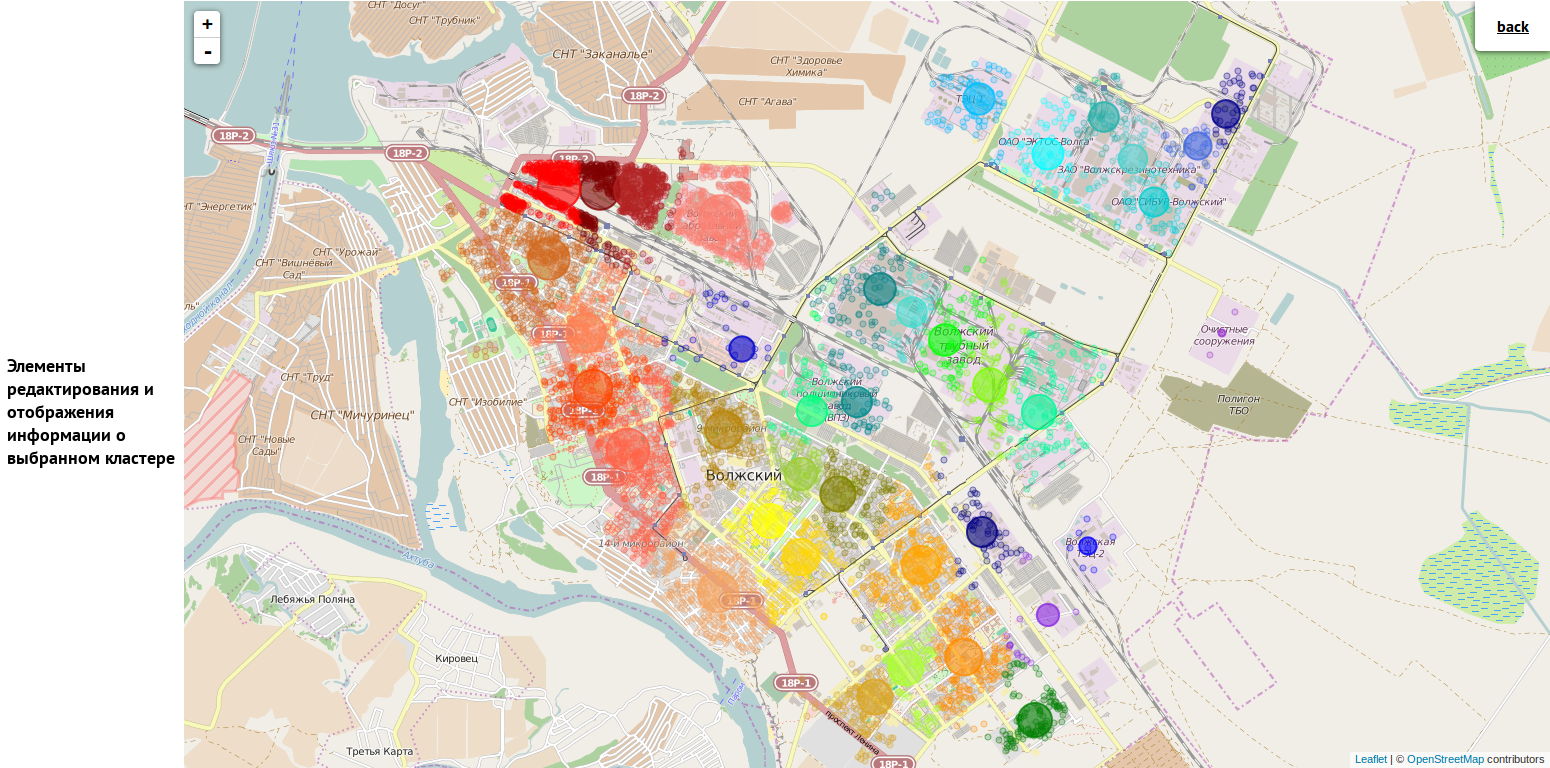
\includegraphics[width=\textwidth]{ui}
\end{figure}

\noindent
\emph{Реализованный алгоритм:} \url{https://github.com/vstu-cad-stuff/clustering}\\
\emph{Текущая реализация:} \url{http://vstu-cad-stuff.github.io/clustering/}\\

\newpage

\section{Псевдокод алгоритма K-Means}\label{ref:kmeans}
\noindent
\begin{enumerate}\itemsep -.5ex
    \item Генерирование начального распределения центроидов
    \item итерация = 0
    \item \textbf{ПОВТОРЯТЬ}
    \item Рассчет принадлежности всех точек центроидам
    \item Рассчет нового положения центроидов
    \item Сдвиг центроидов
    \item итерация += 1
    \item \textbf{ПОКА} разница между рассчитанным положением и текущим не равна 0 и пока
        количество итераций не достигло максимума
    \item \textbf{ВЫВОД} центроиды
\end{enumerate}

\section{Псевдокод алгоритма Mean Shift}\label{ref:meanshift}
\noindent
\begin{enumerate}\itemsep -.5ex
    \item Генерирование начального распределения центроидов
    \item \textbf{ПОВТОРЯТЬ}
    \item Определение соседних точек к центроидам
    \item Определение среднего веса соседних точек к центроидам
    \item Рассчет нового положения центроидов
    \item Сдвиг центроидов
    \item \textbf{ПОКА} разница между рассчитанным положением и текущим не будет равна 0
    \item \textbf{ВЫВОД} центроиды
\end{enumerate}
